\documentclass[12pt]{article}
\usepackage{classlog} % see geometry.pdf on how to lay out the page. There's lots.
%\usepackage{geometry} % see geometry.pdf on how to lay out the page. There's lots.
\usepackage[left=2cm, right=2cm, top=2cm]{geometry}
\geometry{a4paper} % or letter or a5paper or ... etc
\usepackage{graphicx}
% \geometry{landscape} % rotated page geometry
% See the ``Article customise'' template for come common customisations
\usepackage{amssymb}
\usepackage{imakeidx}
\usepackage[italian]{babel}
\usepackage{fancyvrb}
\usepackage{tikz}
\usepackage{wrapfig}

%\usepackage{lgrind}
\usetikzlibrary{arrows,shapes,backgrounds}
\usepackage{framed}
\usepackage{enumerate}

\renewenvironment{shaded}{%
  \def\FrameCommand{\fboxsep=\FrameSep \colorbox{shadecolor}}%
  \MakeFramed{\advance\hsize-\width \FrameRestore\FrameRestore}}%
 {\endMakeFramed}

\newcommand*{\mysep}[1]{%
 \noindent\rule{\textwidth}{1pt}%
}

\newcommand*{\prosep}[1]{%
 \noindent\rule{\textwidth}{0.75pt}%
}
\usepackage{lab}

\DefineVerbatimEnvironment{coding}{Verbatim}%
    {showspaces,showspaces,fontsize=\footnotesize,commandchars=\\\{\}}% showspaces and showtabs only for visualizing

\pagestyle{empty}

%%% BEGIN DOCUMENT
\begin{document}
%\maketitle

%\pagenumbering{arabic} 
\pagestyle{empty}

\begin{labheader}{Fondamenti di Informatica $\diamond$ 2019-20}{5}{05-12-2019}
\end{labheader}

\begin{labex}{Tag Cloud o Word Cloud}\end{labex}

\begin{wrapfigure}{r}{0.45\textwidth}
  \begin{center}\vspace{-2em}
    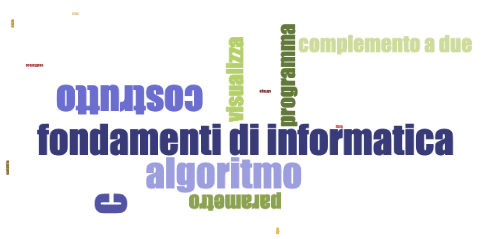
\includegraphics[width=\linewidth]{wcex.png}
  \end{center}%\vspace{-6em}
\end{wrapfigure}

Si vuole realizzare un programma che partendo da un file di testo crei una cosiddetta \textit{Word Cloud} da visualizzarsi mediante una pagina web. Per raggiungere lo scopo, sono dati i seguenti file di testo (disponibili su \texttt{piazza.com}):\begin{itemize}
\item \texttt{stopWords.it.txt} e \texttt{stopWords.txt} che contiene le parole che non vanno considerate in quanto non rilevanti dal punto di vista della semantica (ad esempio congiunzioni, articoli, ...) sia per la lingua italiana che per quella inglese,
\item \texttt{d3.layout.cloud.js}, \texttt{d3.min.js} e \texttt{word-cloud.js} file javascript utilizzati dalla pagina web per realizzare la Word Cloud, e
\item \texttt{wordcloud.htm} pagina html utilizzata per visualizzare la Word Cloud, che include la seguente direttiva: 
\begin{verbatim}
<script type="text/javascript" src="words.js"></script>
\end{verbatim}
Il file \texttt{words.js} \`e ci\`o che il programma deve creare per ottenere il risultato desiderato.
\end{itemize}

Il programma riceve in ingresso un file ASCII contenente il testo da analizzare e crea il file \texttt{words.js} risultato dell'analisi. Il formato di tale file \`e il seguente:
\begin{verbatim}
var tags = [
{"key": "programma", "value" : 26},
{"key": "C", "value" : 27},
{"key": "variabile", "value" : 25},
{"key": "ciclo", "value" : 25},
{"key": "costrutto", "value" : 27},
{"key": "tipo", "value" : 25},
{"key": "sottoprogramma", "value" : 24},
{"key": "parametro", "value" : 26},
{"key": "visualizza", "value" : 26},
{"key": "argc", "value" : 25},
...
{"key": "lista", "value" : 6}
];
\end{verbatim}

A parte la prima e l'ultima riga, ogni elemento specifica un vocabolo quante volte compare nel testo.

Nel realizzare la soluzione, si tengano presente i seguenti aspetti:
\begin{itemize}
\item non mettere nel file finale i vocaboli che compaiono meno di 6 volte;
\item tutti i vocaboli hanno al pi\`u 30 caratteri (simbolo \texttt{LEN}); 
\item i vocaboli contenuti nei file \texttt{stopWords.it.txt} e \texttt{stopWords.txt} sono tutti minuscoli;
\item i vocaboli nel file da analizzare possono avere maiuscole, si tratta di un testo reale;
\item nel file da analizzare ci possono essere segni di interpunzione (virgola, apostrofo, ...) e devono essere opportunamente gestiti;
\item il file da analizzare potrebbe contenere doppi spazi, trovare i vocaboli 
\end{itemize}

A titolo di esempio di ci\`o che dovrebbe realizzare il programma si consideri il testo inziale qui riportato
\vspace{0.5em}
\begin{quotation}
[...] Ai tempi in cui accaddero i fatti che prendiamo a raccontare, quel 
borgo, gi\`a considerabile, era anche un castello, e aveva perci\`o l'onore 
d’alloggiare un comandante, e il vantaggio di possedere una stabile 
guarnigione di soldati spagnoli, che insegnavan la modestia alle fanciulle 
e alle donne del paese, accarezzavan di tempo in tempo le spalle a qualche 
marito, a qualche padre; e, sul finir dell’estate, non mancavan mai di 
spandersi nelle vigne, per diradar l'uve, e alleggerire a' contadini le fatiche 
della vendemmia. Dall'una all'altra di quelle terre [...]
\end{quotation}
\vspace{0.5em}
i vocaboli che il programma dovrebbe considerare, prima di aver ignorato quelli presenti nel file \texttt{stopWords.it.txt} sono:
\vspace{0.5em}
\begin{quotation}
[...] ai tempi in cui accaddero i fatti che prendiamo a raccontare quel borgo gi\`a considerabile era anche un castello e aveva perci\`o onore alloggiare un comandante e il vantaggio di possedere una stabile guarnigione di soldati spagnoli che insegnavan la modestia alle fanciulle e alle donne del paese accarezzavan di tempo in tempo le spalle a qualche marito a qualche padre e sul finir estate non mancavan mai di spandersi nelle vigne per diradar uve e alleggerire contadini le fatiche della vendemmia una altra di quelle terre [...]
\end{quotation}\vspace{0.5em}
utilizzando il file \texttt{stopWords.it.txt}, il programma scarter\`a i vocaboli che compaiono in tale file, arrivando ai seguenti vocaboli (non \`e importante che non ci siano vocaboli ripetuti)
\vspace{0.5em}
\begin{quotation}
tempi fatti prendiamo raccontare borgo considerabile castello onore alloggiare comandante vantaggio possedere stabile guarnigione soldati spagnoli insegnavan modestia fanciulle donne paese accarezzavan tempo tempo spalle marito padre finir estate  mancavan spandersi vigne diradar uve alleggerire contadini fatiche vendemmia terre
\end{quotation}
\vspace{1em}

Si utilizzi il seguente tipo di dato:
\begin{lstlisting}[language=C,numbers=none]
typedef struct wordlist_s {
	char word[LEN+1];
	int times;
	struct wordlist_s * next;
} wordlist_t;
\end{lstlisting}

Si considerino gi\`a a disposizione i seguenti sottoprogrammi (codice disponibile su \texttt{piazza.com}):

\begin{itemize}
\item 
\begin{lstlisting}[language=C]
wordlist_t * increasing(wordlist_t * h, char * w);
\end{lstlisting} 
inserisce un nuovo elemento in ordine alfabetico crescente rispetto al campo \texttt{word} della struttura;
\item
\begin{lstlisting}[language=C]
wordlist_t * deleteptr(wordlist_t * h, wordlist_t * e)
\end{lstlisting} 
elimina un elemento dalla lista;
\item 
\begin{lstlisting}[language=C]
wordlist_t * find(wordlist_t * h , char * w);
\end{lstlisting} 
 trova e restituisce della lista con un certo valore nel campo \texttt{word} della struttura, se esiste, altrimenti restituisce \texttt{NULL}.
\end{itemize}

Si utilizzino i sottoprogrammi delle librerie \texttt{string.h}, \texttt{stdlib.h}, \texttt{ctype.h} e simili quando utili, senza sviluppare ex-novo cose che gi\`a esistono.

\getsol{srccode/wordcloud.c}





\end{document}